%% -----------------------------------------------------------------------------

Trails and their properties provide the tools for a rigorous examination of
blame for Natural, Transient and Erasure. In line with the discussion so far,
the test bed collects data to answer three initial questions for 
interesting debugging scenarios:
\begin{itemize}
\item[$Q_1$] Is blame useful in the context of Natural?

\item[$Q_2$] Is first blame useful in the context of Transient?

\item[$Q_3$] Is last blame useful in the context of Transient?

\end{itemize}

Furthermore, the experiment allows a comparison of the relative usefulness of blame
information:
\begin{itemize}
\item[$Q_*$] Is blame for X more useful than blame for Y (for X, Y in Natural, Transient, or Erasure)?
\end{itemize}

\begin{figure}[ht] \footnotesize
\center
{\begin{tabular}{l|c|c|c}
%% ---------------------------------------------------------------------------------------------------------------
                        & {\bf Natural}  & {\bf Transient} &  {\bf Erasure} \\ \hline 
%% ---------------------------------------------------------------------------------------------------------------
{\bf Blame}             &  $Q_1/Q_*$    &                  &                \\
{\bf First blame}       &               &     $Q_2/Q_*$    &                 \\
{\bf Last blame}        &               &     $Q_3/Q_*$    &                 \\
{\bf Exceptions}        &      $Q_1$    &     $Q_2/Q_3$    &      $Q_*$      \\
\end{tabular}}
  \label{fig:experiment-outline}
\end{figure}

The above table summarizes how each question relates to
different kinds of trails/modes of the rational programmer. For example,
experimental question $Q_1$ asks whether blame is valuable for Natural and the
experiment uses the Natural blame and exception trails to answer it, so $Q_1$
shows up in the cells for Natural blame and Natural exceptions.

%% -----------------------------------------------------------------------------

In detail, the answer to $Q_1$ demands a comparison of the success of the Natural
blame and Natural exception trails for all debugging scenarios.  The
first step is to construct each mutant's scenario lattice and identify their
debugging scenarios.  The test bed then extends the trails that start
from those roots according to the Natural-blame programmer.  If no scenarios can
be added to the trail, the test bed checks whether the last scenario
of the trail type-checks or not. If it does, the
Natural-blame trail is successful; otherwise it is failing. 
Figure~\ref{fig:process} summarizes this experimental process for
one mode of the rational programmer and connects it with the mutations from
section~\ref{sec:mutate}.
The process is repeated for the same roots with the other mode, Natural
exceptions.
After completing, the test bed
reports the success/failure results of the trails to determine the proportion of
scenarios where Natural blame is more useful than Natural exceptions.  Question
$Q_1$ has a positive answer if a root exists where the above is true because it
is evidence that there is at least one interesting scenario that the rational
programmer manages to debug because of blame information.  The process is analogous
for $Q_2$ and $Q_3$, using the respective modes of the rational programmer.

\begin{figure}[bh] \footnotesize
  \centering
  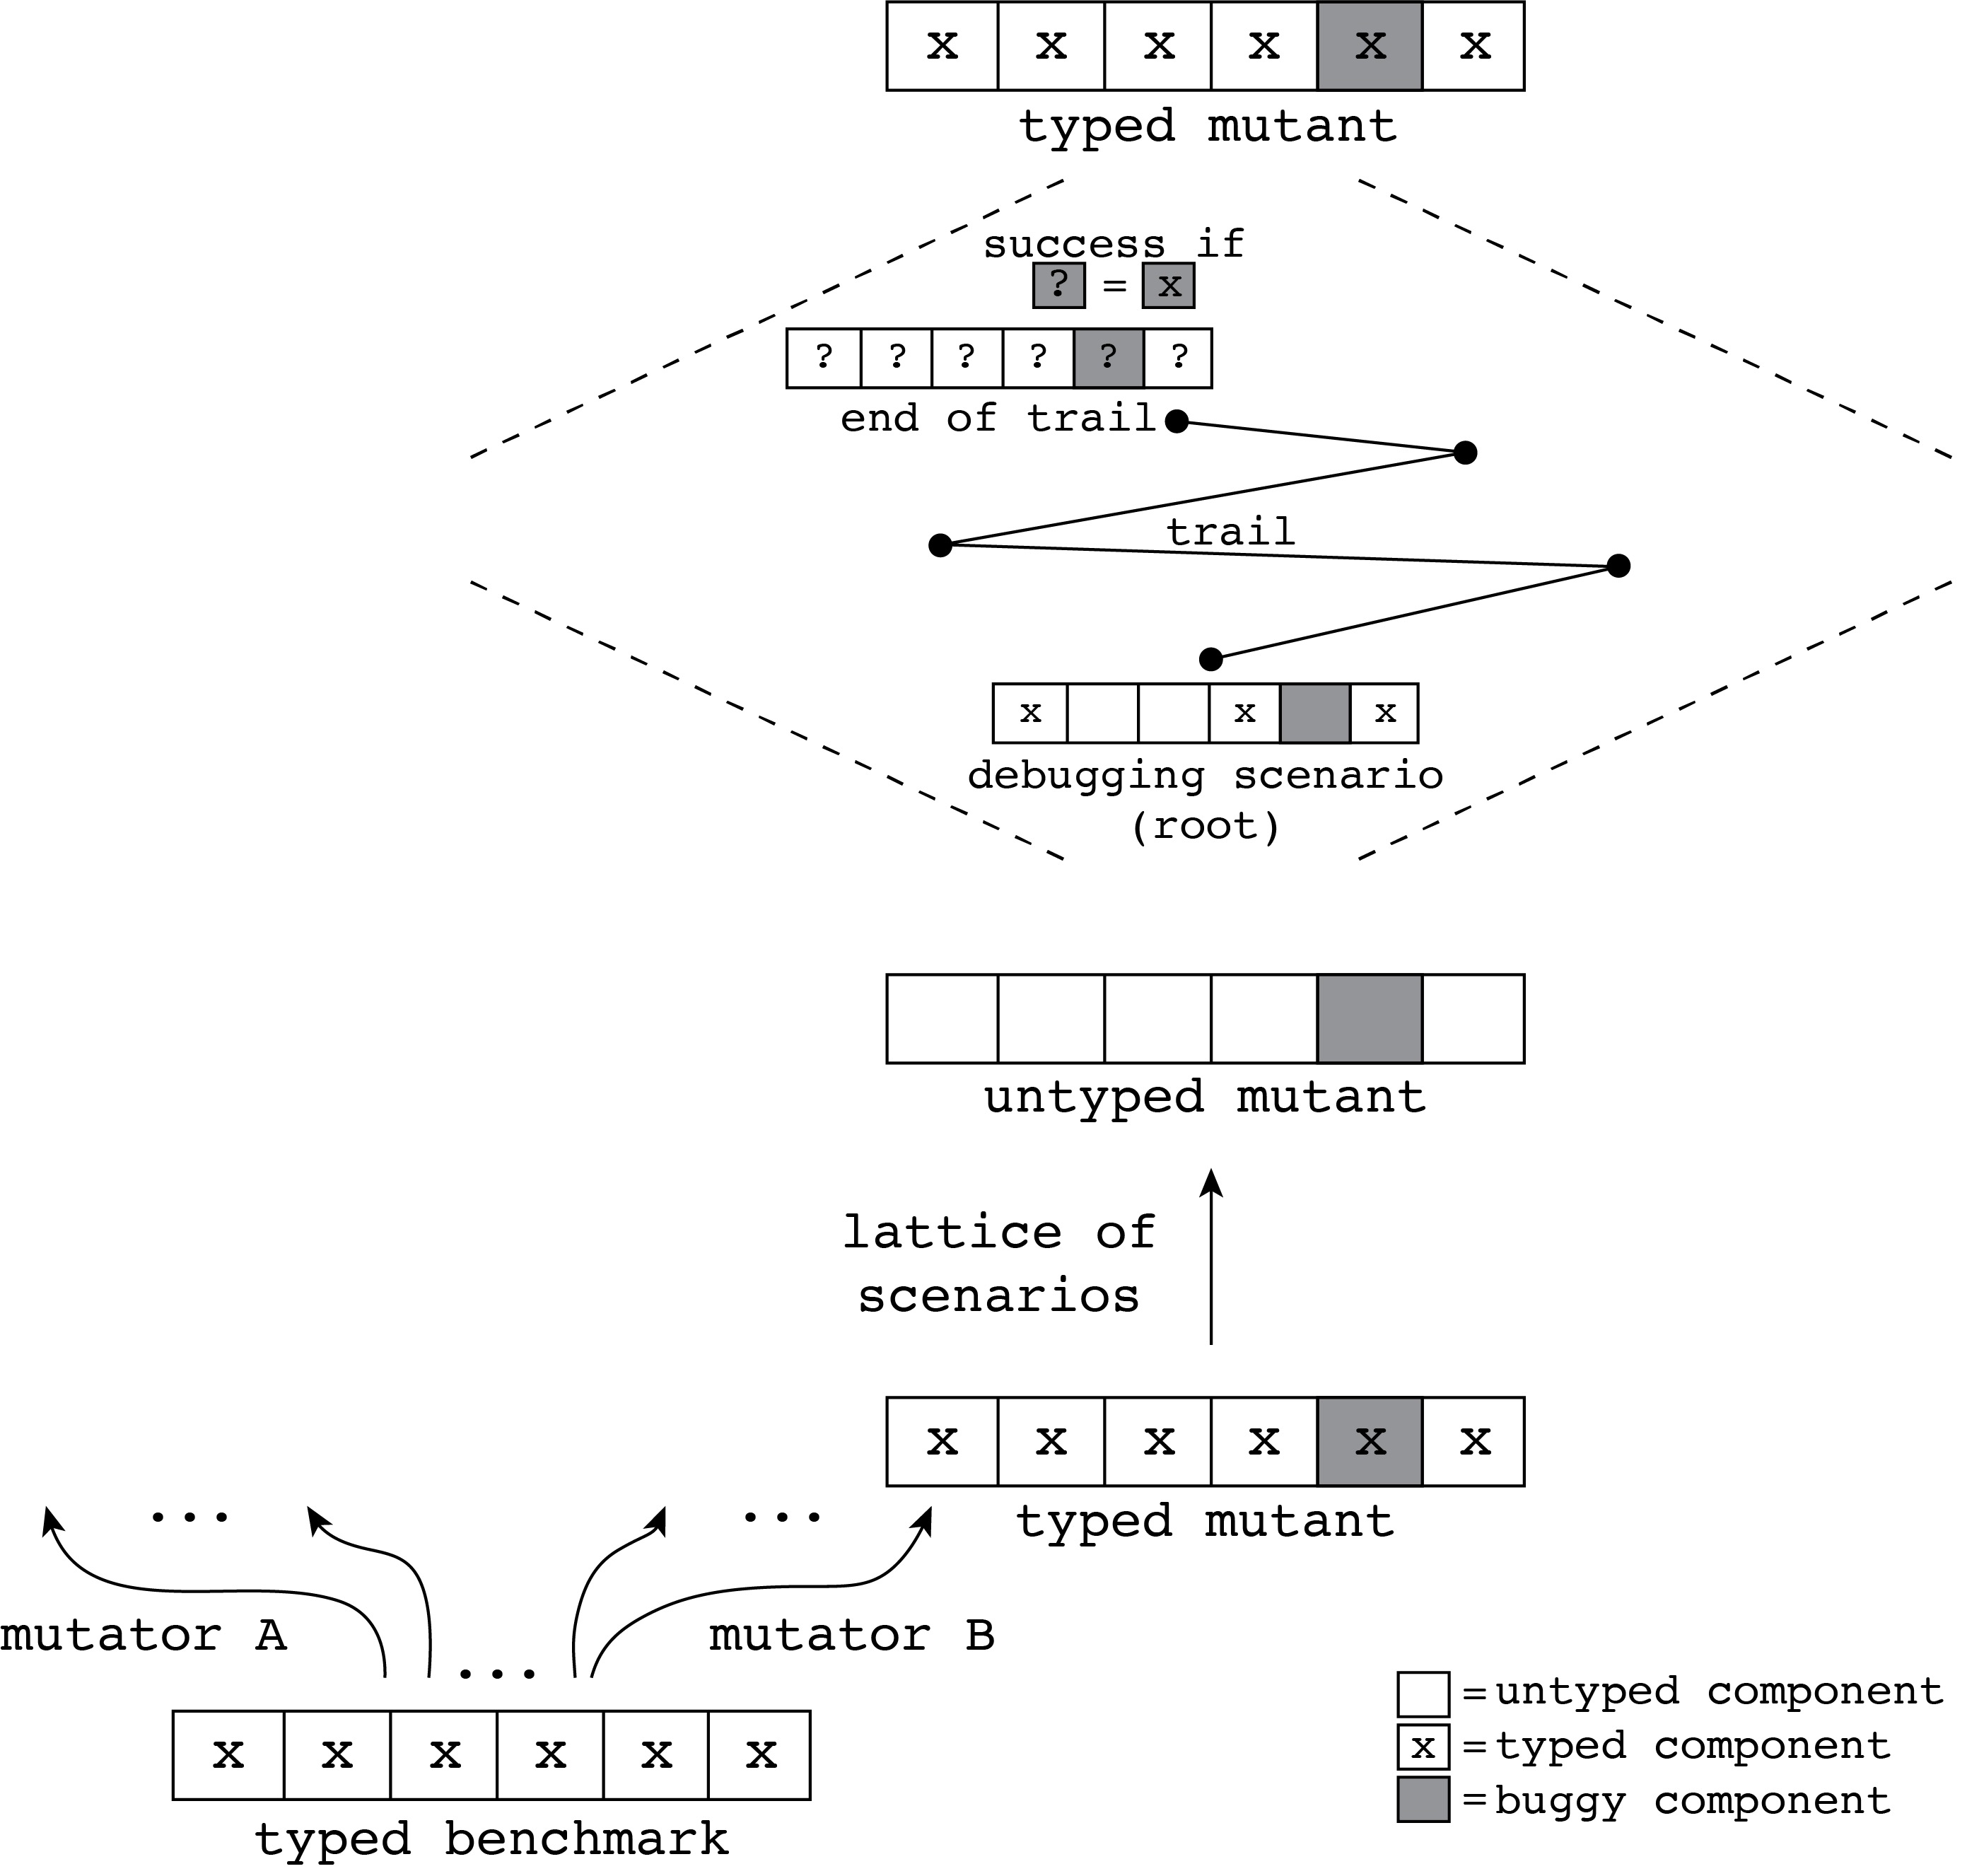
\includegraphics[scale=0.36]{./Images/process}
  \caption{The experimental process for one mode of the rational programmer}
  \label{fig:process}
\end{figure}


For $Q_*$, the process is a bit more involved. Answering this question calls for
a comparison of the percentage of scenarios where one mode is more useful than
the other and the inverse.  For instance, deciding whether blame for Natural is
more useful than first blame for Transient requires comparing the percentage
of scenarios where Natural blame is more successful than Transient
first blame with the percentage where Transient first
blame is more successful than Natural blame. Repeating the whole process
for every pair of modes produces a
complete picture of the comparative usefulness of blame between all of the modes.


